\let\mypdfximage\pdfximage
\def\pdfximage{\immediate\mypdfximage}
\documentclass[11pt]{article}

\usepackage{bridges}
\usepackage{rotating} %% For the sideways
\usepackage{graphicx} %% For including pretty pictures
\usepackage{url}      %% For formatting URLs.
\usepackage{amsmath}  %% for \text
\usepackage{amssymb}  %% for the square

\title{\textbf{People and Computers Agree on the Complexity of Small Art}}

\author{
	Peter Boothe \\
	Google, New York, NY \\
	Manhattan College, Riverdale, NY \\
	\url{pboothe@gmail.com} \\
	\\
	Jonathan Langke \\
	Manhattan College, Riverdale, NY \\
	\url{jlangke22@gmail.com}
}

\date{}


\bibliographystyle{plain}

%% Set the indentation at the start of paragraphs.
\setlength{\parindent}{0.3in}

%% Set the spacing between paragraphs.  The guidelines don't specify
%% that there should be a space, but I find paragraphs hard to read
%% without it.  I'm inserting a small space that you may choose to
%% modify.
\setlength{\parskip}{.75ex}

\begin{document}
\maketitle

%% Make sure not to include a page number on the first page.
\thispagestyle{empty}

\begin{abstract}

Restricting our purview to black and white digital artworks on a grid, we
developed a lower-power version of Kolmogorov complexity, and then we found the
complexity of every piece of 3x3 art.  We also asked people to compare two
artworks and decide which one was more visually complex as they understood the
term.  We used these comparisons to assign every artwork a strength rating
(similar to a chess rating), and we found that the human-generated ratings were
well correlated with the formula complexity of the artworks.  Therefore,
computers and humans largely agree on the complexity of small artworks!

\end{abstract}

\section*{Introduction}

We compare the complexity of small artworks from two perspectives: that of a
computer, and that of a human.  To do this in a principled manner we define our
artworks, define our notion of complexity for computers, and describe how we
measured visual complexity for people.  We procede through each task in turn,
one per section, before bringing our computer and human results
together and describing future work in the last sections.

\section*{Our Definition of Art}

In order to make this question tractable, and in order to ensure that our
artworks are ``native'' to both the human and computer domains, we restrict our
purview to black and white pixel-based digital artworks.  This is clearly a
subset of all digital artworks, but it is still an expressive subset, as shown
in Figure~\ref{fig:monalisa}.  

We can generate a mapping of positions on the grid to black and white pixels in
multiple ways.  The simplest way to generate the mapping is to simply write
down the sequence verbatim.  However, considered more generally, each artwork
can also be thought of as the output of a function that takes two numbers as
input (representing the grid position of each pixel) and returns either true or
false (representing whether the pixel at that position is black or white).  In
computer science terms, every black and white picture is the output of a
function of type {\tt int$\times$int$\to$bool}.  

\begin{figure}
\begin{center}
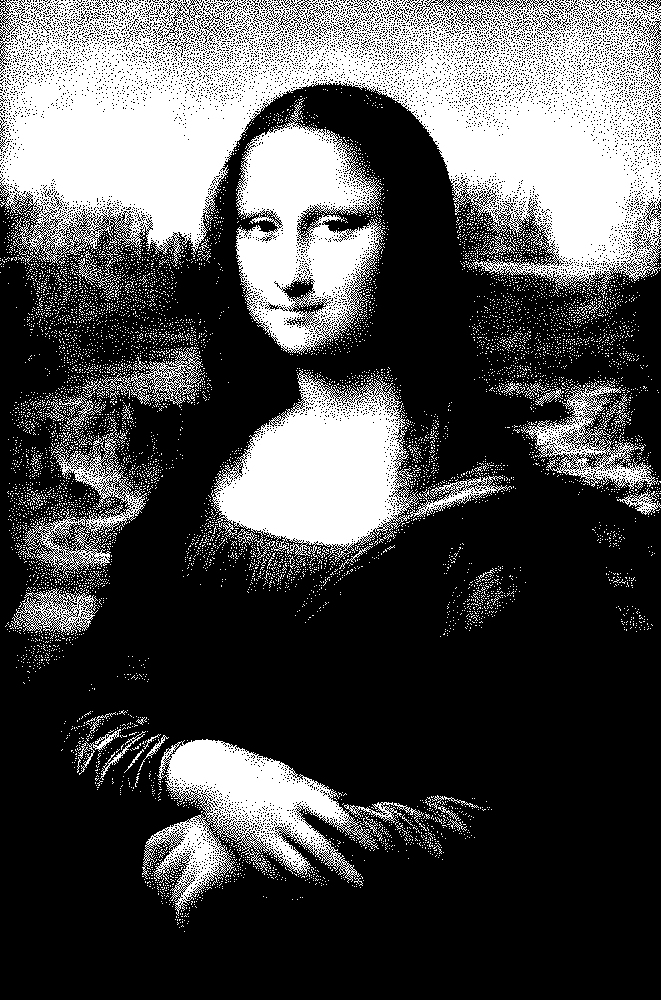
\includegraphics[width=5in]{monalisa_mono.jpg}
\end{center}
\caption{A example artwork consisting of black and white (and no gray) pixels on a grid.}
\label{fig:monalisa}
\end{figure}

This isomorphism between functions of type {\tt int$\times$int$\to$bool} and
black and white artworks is the basis of our work, as it allows us to ask
people about the perceived visual complexity of an artwork, and to ``ask''
computers about the complexity of the corresponding functions.  In order to
make our problems computationally tractable, we restrict our purview to
artworks that are nine pixels laid out in a three by three grid.  This allows
us to generate all artworks (of which there are $2^9=512$), and also, less
trivially, to enumerate all possible formulae in an effort to calculate the
formula complexity of each artwork.

\section*{Formula Complexity}

Formula complexity is intended to be a ``low power'' version on Kolmogorov
complexity\footnote{Also called Chaitin-Kolmogorov complexity.  The standard
text is Li and Vit\'anyi\cite{Li}, although Chaitin's article in
Scientific American\cite{chaitin} provides a very approachable introduction.}.  In
Kolmogorov complexity, the complexity of an object is defined to be the size of
the smallest program that outputs that object --- interestingly, the
programming language used does not usually matter, as all Turing-complete
programming languages are equivalent up to an additive constant.

Formula complexity is also a property of an object, in this case a
2-dimensional artwork, but the programming language used to write the function
of type {\tt int$\times$int$\to$bool} is not Turing-complete.  In particular,
in formula complexity it is impossible to define and call functions, which
prohibits looping and recursion.  Instead of the entirety of mathematical
symbols, in formula complexity we restrict ourselves to just the symbols in the
set \[\{\text{\tt +, *, 0, 1, x, y, true, false, not, and, or, <}\}.\] We also
require that every expression be fully parenthesized, to eliminate any
potential ambiguity of interpretation.  In each formula {\tt x} and {\tt y}
represent the coordinates of the grid point being interpreted.  

Note that some formulae that our language can produce might make no sense.  For
example, what is the value of {\tt (1 + false)}?  Furthermore, other formulae
produced may make sense, but not be useful in our context.  For example, if our
formula is {\tt (x + y)}, then what color should we make the pixel at $(1,0)$?
Therefore, we place further restrictions on our formulae:
\begin{enumerate}
\item All formulae must be well-typed: numerical operations are only performed
on numbers (or subexpressions which evaluate to a number) and logical operations
are only performed on logical values (or subexpressions which evaluate to a
logical value).
\item All formulae must evaluate to {\tt true} or {\tt false} after
substituting the coordinate values in for {\tt x} and {\tt y}.
\end{enumerate}
The first requirement ensures that a formula makes sense, and the second
ensures that the formula can be used to define an artwork.  Now that these
preliminaries are decided, we can define formula complexity.

\textbf{Definition (Formula Complexity)}~~The \emph{formula complexity} of an
artwork is the number of symbols used in the smallest formula which produces
that artwork when evaluated at each point on the grid.  

Some example artworks,
along with their formula complexity and the corresponding formula of minimum
size may be seen in Figure~\ref{fig:artexamples}. 

\begin{figure}
\begin{tabular}{cp{.75in}r}
Artwork & Formula Complexity & Formula of minimum size \\
\hline
\reflectbox{\rotatebox[origin=c]{180}{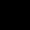
\includegraphics[width=.75in]{3x3pics/0.png}}} & 1 & {\tt true } \\
\reflectbox{\rotatebox[origin=c]{180}{
\includegraphics[width=.75in]{3x3pics/500.png}}} & 5 & {\tt (1 < (x + y))} \\
\reflectbox{\rotatebox[origin=c]{180}{
\includegraphics[width=.75in]{3x3pics/122.png}}} & 16 & {\tt ((not (x < (x * y))) and ((x * x) < (x + (x + y))))}

\end{tabular}
\caption{Some example artworks, listed with their formula complexity and a formula with that complexity.  Black corresponds to false and gray to true, and the bottom left corner pixel $(0,0)$.}
\label{fig:artexamples}
\end{figure}

We wrote a program to generate all well-typed formulae in order of size, and
then tested each formula as it was generated in order to determine if it was
the first formula to produce its corresponding picture.  We ran our program for
months, but were only able to generate the formulae up to size 17 due to the
extremely large number of formulae and the super-exponential explosion in
formula count as formula size grows.  A complete diagram of all artworks with
their corresponding formula complexity may be seen in
Figure~\ref{fig:allthe3x3}.

\begin{figure}
\begin{center}
\begin{sideways}
\input{3x3table.tex}
\end{sideways}
\end{center}

\caption{All the three by three artworks and the formula complexity of each.  The last category is labeled $\ge 17$ because the formula complexity of those artworks is unknown, except that it is at least 17.}
\label{fig:allthe3x3}
\end{figure}

\section*{Visual Complexity}

When compared with the mathematical formalism of formula complexity, visual
complexity is a frustratingly slippery concept.  We declined to define it at
all, instead allowing every survey participant to decide for themselves what it
meant.  We surveyed people online (through Twitter and through our own social
networks) and presented them with a page that showed two artworks and asked
them to click on the artwork that was more visually complex.  After they
clicked on one artwork, we presented them with another, and another, until
they decided for themselves to stop taking our survey.

Our task was then to distill these ratings into a ranking of visual complexity.
We did this by treating each survey response as a ``game result'' between the
two artworks and then turned the win-loss record of each artwork into a
strength rating using the TrueSkill algorithm\cite{trueskill}, which is a
rating system similar to the one used in chess but with provably better
convergence times\footnote{The TrueSkill algorithm was developed at Microsoft
and is currently used to rank players in XBox Live.}.

\section*{Comparing Complexity Results}

Armed with our computational results and our survey results, the only thing
left to do was see whether these two complexity rankings were well-correlated!
A complete chart of our results may be seen in Figure~\ref{fig:scatter}.  From
the figure, two things are clear: First, our correlation is definitely not
perfect because the dots do not form an increasing line; Second, there is some
correlation, because there are very few dots in the lower right or in the upper
left.

\begin{figure}
\begin{center}
\includegraphics[width=5in]{3x3scatter.pdf}
\end{center}
\caption{A scatter plot comparing visual complexity and formula complexity for
all 512 artworks, along with the line of best-fit.  The formula complexity is
artificially clamped at 17.  The correlation coefficient between the two
measurements is $.55$ and the p-value is $4\cdot10^{-39}$.} 
\label{fig:scatter}
\end{figure}

When we calculate Pearson's correlation coefficient, we get a correlation of
$.55$ and a very low p-value of $4\cdot10^{-39}$, which implies that it is safe
to reject the null hypothesis that these two distributions have nothing to do
with one another.  After rejecting the null hypothesis we can safely conclude
that, for small digital artworks, visual complexity is positively correlated
with formula complexity!  

\section*{Conclusion and Future Work}

We defined a class of art that is explicable by both humans and computers.  We
also defined a ``powered down'' version of Kolmogorov complexity which we
called formula complexity and calculated the formula complexity of all 3x3
artworks.  We then took survey results where we asked people to compare these
artworks to each other and choose the one that is most complex, and we assigned
a complexity rating to each artwork based on the number of comparisons it won
and the strength of the artworks it beat.  We then showed that these two, very
different, complexity measures are actually highly correlated.  From all this,
we conclude that, for small digital artworks, humans and computers agree
about what is complex and what is simple!

The future work we lay out is related to the limits of both of our complexity
surveys, potential ways of increasing the power of our computer complexity
measure, and a search for a computer complexity measure that comes even closer
to the human one.

Our computational survey was unfortunately limited by available machine power.
It may be fruitful to run this computation again in a few years once transistor
density has increased again.  Perhaps future programmers could find the formula
complexity of all of the small artworks!

Our human survey was limited to college students and Twitter friends.  Because
we are computer scientists, it is likely that the college students and Twitter
users we know are not representative of the population at large.  Does this
correlation increase as when people take computer science classes?  Are we only
seeing a correlation because we surveyed people who had taken CS classes? 

Our complexity measure of formula complexity was partly driven by expediency
and explicability.  Other areas of math and CS have developed programming
languages and formula schema that allow for richer expressions than we have
here.  For example, it might be interesting to replicate this result using the
simply-typed lambda calculus, which allows function definition and just forbids
recursion.  For another example, it might be interesting to replicate this
result using Levin complexity, which is even closer to Kolmogorov complexity!

Finally, and most interestingly, it could be quite fruitful to search for the
set of atoms which provide for a formula complexity that maximally matches the
measured visual complexity.  The discovery of this set of atoms would
potentially have deep implications for understanding how human brains perceive
the world.

\bibliography{bibliography} 
\end{document}
